%==============================================================================
% Financial Fraud Detection - Analysis Report (LaTeX template)
% Compile from the reports/ directory so figure paths resolve:
%   cd reports && pdflatex analysis_report.tex && pdflatex analysis_report.tex
% (run twice so the table of contents / references resolve)
%==============================================================================
\documentclass[11pt,a4paper]{article}

\usepackage[utf8]{inputenc}
\usepackage[T1]{fontenc}
\usepackage{lmodern}
\usepackage[margin=1in]{geometry}
\usepackage{graphicx}
\usepackage{booktabs}
\usepackage{array}
\usepackage{float}
\usepackage{caption}
\usepackage{xcolor}
\usepackage{amsmath}
\usepackage{fancyhdr}
\usepackage{enumitem}
\usepackage[colorlinks=true,linkcolor=blue!60!black,urlcolor=blue!60!black]{hyperref}

\definecolor{accent}{HTML}{C0392B}
\captionsetup{font=small,labelfont=bf}
\graphicspath{{figures/}}   % look for images in reports/figures/

% ---- header / footer ----
\pagestyle{fancy}
\fancyhf{}
\lhead{\small Financial Fraud Detection}
\rhead{\small Analysis Report}
\cfoot{\thepage}
\renewcommand{\headrulewidth}{0.4pt}

% ---- title ----
\title{\textbf{Financial Fraud Detection}\\[0.3em]
       \large Full Analysis Report}
\author{Naman}
\date{2026-06-09 \quad\textbar\quad Dataset: ULB Credit Card Fraud (Kaggle)}

\begin{document}
\maketitle
\thispagestyle{fancy}

\begin{abstract}
\noindent We build an end-to-end machine-learning pipeline to detect fraudulent
credit-card transactions in a severely imbalanced dataset (\textbf{0.17\% fraud}).
After cleaning, leak-safe preprocessing, exploratory analysis and a four-model
comparison, \textbf{XGBoost} is the best classifier (\textbf{PR-AUC 0.82}). We tune
the decision threshold against an explicit cost model and recommend operating at a
\textbf{0.12 threshold}, catching \textbf{$\sim$84\% of fraud} and lowering estimated
fraud cost \textbf{$\sim$20\%} versus the naive 0.50 default. Throughout we measure
\textbf{recall and PR-AUC rather than accuracy}, which is meaningless at this level
of imbalance.
\end{abstract}

\begin{table}[H]
\centering
\caption{Headline results}
\begin{tabular}{@{}ll@{}}
\toprule
\textbf{Metric} & \textbf{Value} \\
\midrule
Transactions analysed (post-dedup) & 283,726 \\
Confirmed fraud & 473 (0.17\%) \\
Best model & XGBoost (PR-AUC 0.82, ROC-AUC 0.97) \\
Recommended threshold & 0.12 (cost-optimal) \\
Fraud caught at recommendation & 84\% (recall) \\
Estimated cost reduction vs default & $\sim$20\% \\
\bottomrule
\end{tabular}
\end{table}

\clearpage
\tableofcontents
\clearpage

%------------------------------------------------------------------------------
\section{Objective}
Detect fraudulent transactions and translate the model into an actionable,
cost-aware business decision --- not just a classifier but a recommendation a
fraud-operations team could act on. Success is measured by the ability to catch
fraud (\emph{recall}) while keeping false alarms manageable (\emph{precision}),
and by framing the trade-off in money.

%------------------------------------------------------------------------------
\section{Data and Methodology}
The dataset contains 284,807 European card transactions over two days. Features
are \texttt{Time}, \texttt{Amount}, a \texttt{Class} label (1 = fraud) and
\textbf{V1--V28} --- principal components published in place of the raw features
for privacy.

\paragraph{Pipeline (modular, leak-safe by design).}
\begin{quote}
\texttt{load $\rightarrow$ clean (dedup) $\rightarrow$ SPLIT (stratified)
$\rightarrow$ scale (fit on train only) $\rightarrow$ handle imbalance (train only)
$\rightarrow$ train 4 models $\rightarrow$ evaluate on test $\rightarrow$ tune
threshold by cost}
\end{quote}
The cardinal discipline: \emph{anything that learns from data (scaler statistics,
SMOTE) sees the training set only.} The test set stays an untouched
$\sim$0.17\%-fraud sample, so every reported number reflects unseen,
production-like data. This is the most common place fraud projects accidentally
leak and over-report performance.

%------------------------------------------------------------------------------
\section{Data Cleaning}
\begin{itemize}[leftmargin=1.4em]
  \item \textbf{Removed 1,081 exact duplicate rows} --- duplicates can land in
        both train and test, leaking information and inflating scores. 283,726
        rows remained.
  \item \textbf{No missing values}; confirmed no negative amounts.
  \item \textbf{Outliers kept deliberately} --- in fraud the outlier often
        \emph{is} the fraud.
  \item \textbf{Scaled \texttt{Amount} and \texttt{Time} with RobustScaler}
        (median/IQR based, resistant to extremes). V1--V28 are already
        PCA-scaled.
\end{itemize}

%------------------------------------------------------------------------------
\section{Exploratory Analysis}

\subsection{Class imbalance}
Fraud is 0.17\% of transactions. A model predicting ``always legitimate'' scores
99.8\% accuracy and catches nothing --- which is why accuracy is excluded from all
evaluation below.

\begin{figure}[H]
\centering
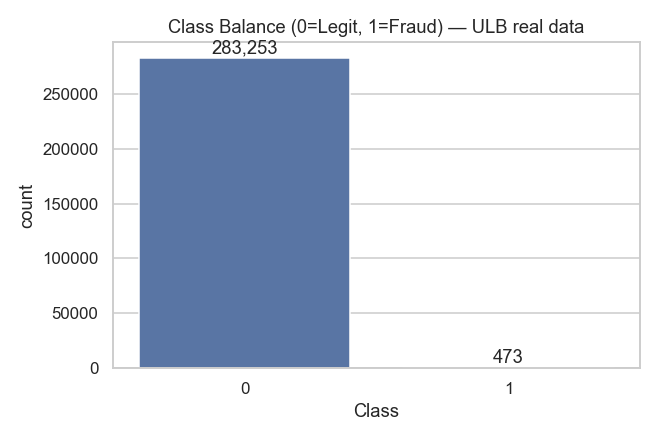
\includegraphics[width=0.55\textwidth]{01_class_balance.png}
\caption{Class balance: 284{,}315 legitimate vs.\ 492 fraud (pre-dedup view).}
\end{figure}

\subsection{Finding 1 --- fraud concentrates at night}
Fraud \emph{rate} spikes in the early hours despite that being the lowest-traffic
period: hour 2 $\approx$ \textbf{1.45\%} ($\sim$8.7$\times$ baseline), hour 4
$\approx$ \textbf{1.04\%} ($\sim$6.2$\times$). A transaction at 2--4\,AM is
materially riskier per dollar.

\begin{figure}[H]
\centering
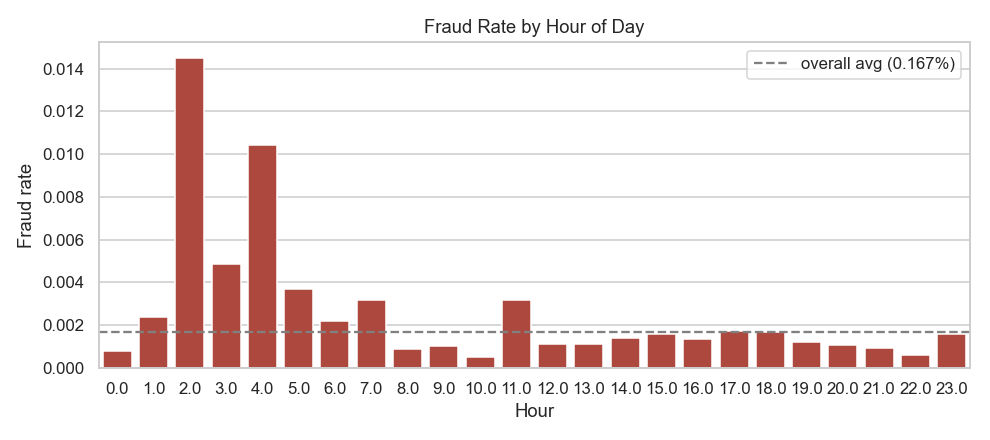
\includegraphics[width=0.8\textwidth]{03_fraud_rate_by_hour.png}
\caption{Fraud rate by hour of day; dashed line is the overall average.}
\end{figure}

\subsection{Finding 2 --- fraud hides in small amounts}
Median fraud amount \textbf{\$9.25} vs.\ \textbf{\$22.00} for legitimate
transactions --- consistent with \emph{card-testing} (a small validating charge on
a stolen card). The fraud \emph{mean} is higher (\$122 vs.\ \$88) only because of a
few large cases, so the median is the honest summary.

\begin{figure}[H]
\centering
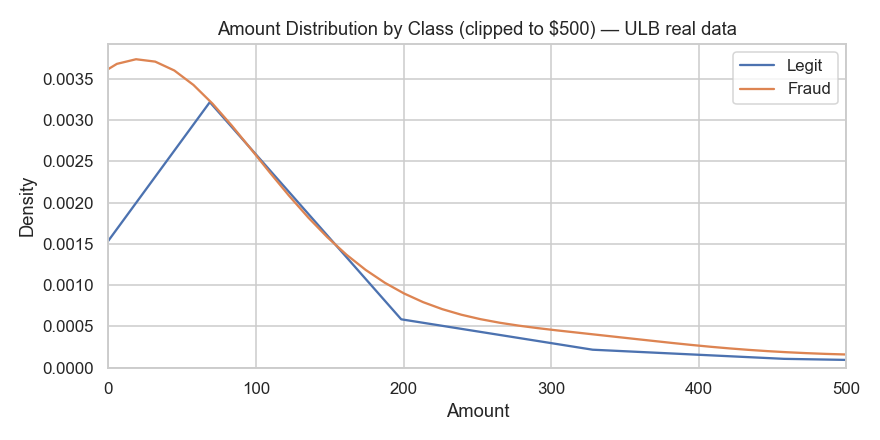
\includegraphics[width=0.8\textwidth]{02_amount_by_class.png}
\caption{Transaction amount distribution by class (clipped for readability).}
\end{figure}

\subsection{Finding 3 --- a few features separate the classes}
V17, V14, V12, V10 correlate most strongly with fraud ($|\text{corr}|$ 0.21--0.31),
all negative, with little distributional overlap --- which is \emph{why} a
classifier can work here. These are PCA components, so we can rank but not
interpret them.

\begin{figure}[H]
\centering
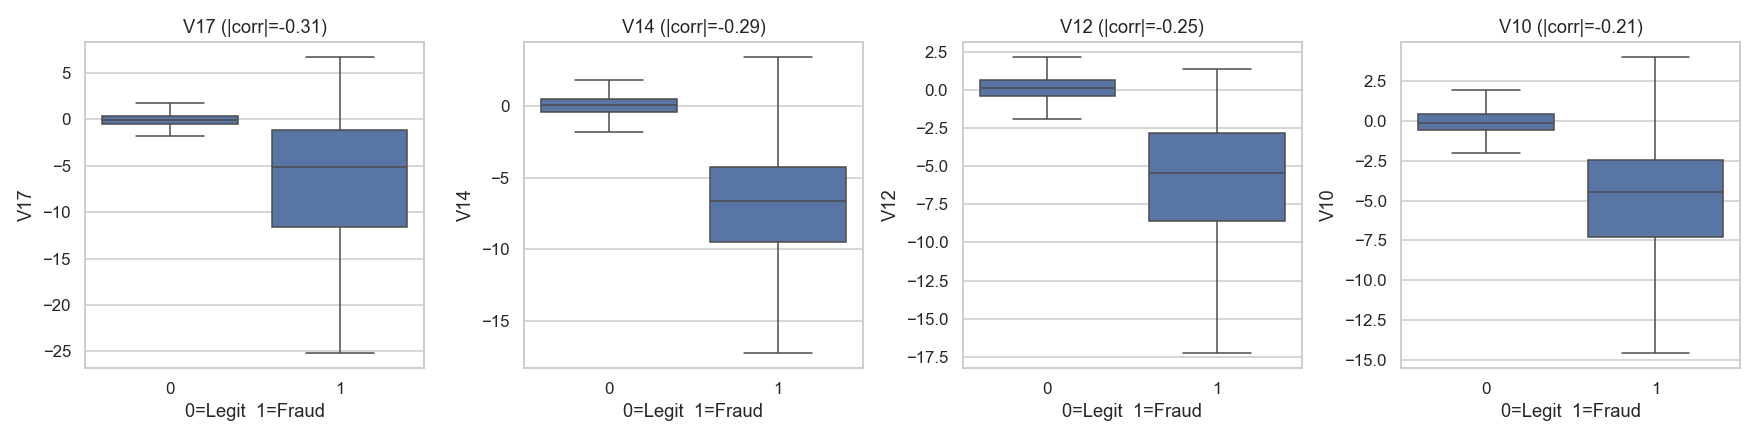
\includegraphics[width=0.95\textwidth]{04_top_feature_boxplots.png}
\caption{Top separating features, fraud vs.\ legitimate.}
\end{figure}

%------------------------------------------------------------------------------
\section{Feature Engineering (and an honest negative result)}
We engineered three interpretable features --- \texttt{Hour}, \texttt{Amount\_log}
and an \texttt{Is\_high\_amount} flag (>99th percentile, threshold learned on train
only). An audit showed weak linear signal, and when we re-trained with them
included they \textbf{did not improve the model and slightly hurt XGBoost
(PR-AUC 0.823 $\rightarrow$ 0.802)}. We therefore \textbf{removed them} and kept the
simpler 30-feature model. This demonstrates disciplined feature selection: low
correlation is not proof of uselessness (time-of-day and rare-event flags are
non-linear), but features that fail to improve held-out performance should not be
retained.

%------------------------------------------------------------------------------
\section{Handling Class Imbalance}
With only $\sim$378 fraud cases in training we compared strategies (applied to
\textbf{train only}): balanced \textbf{class weights} (minority weight $\approx$
300$\times$), XGBoost's native \texttt{scale\_pos\_weight} $\approx$ 600, and
\textbf{SMOTE} oversampling. For the final comparison we used class weights /
\texttt{scale\_pos\_weight} rather than synthesising data, so results reflect
genuine signal.

%------------------------------------------------------------------------------
\section{Model Comparison}
Four models trained and evaluated on the same untouched test set, ranked by
PR-AUC. SVM was trained on a 30{,}000-row subsample for tractability (stated
openly).

\begin{table}[H]
\centering
\caption{Model comparison on the held-out test set (ranked by PR-AUC).}
\begin{tabular}{@{}lrrrrrr@{}}
\toprule
\textbf{Model} & \textbf{Recall} & \textbf{Precision} & \textbf{F1} &
\textbf{ROC-AUC} & \textbf{PR-AUC} & \textbf{Fit (s)} \\
\midrule
\textbf{XGBoost} & 0.789 & 0.862 & 0.824 & 0.966 & \textbf{0.823} & 0.8 \\
Random Forest & 0.716 & 0.971 & 0.824 & 0.945 & 0.808 & 12.1 \\
Logistic Regression & 0.874 & 0.056 & 0.106 & 0.966 & 0.672 & 0.2 \\
SVM (subsample) & 0.484 & 0.414 & 0.447 & 0.937 & 0.474 & 1.7 \\
\bottomrule
\end{tabular}
\end{table}

\paragraph{Why PR-AUC, not ROC-AUC.} Logistic Regression posts a superb ROC-AUC
(0.966) yet a catastrophic precision of \textbf{5.6\%} --- only $\sim$1 flag in 18
is real fraud. ROC-AUC is optimistic under heavy imbalance because true negatives
dominate; PR-AUC exposes the truth. XGBoost wins by balancing recall (79\%) and
precision (86\%).

%------------------------------------------------------------------------------
\section{Evaluation and Threshold Tuning}
A model outputs a probability; the business value lies in \textbf{where we set the
threshold}. The default 0.50 is rarely optimal for fraud.

\begin{figure}[H]
\centering
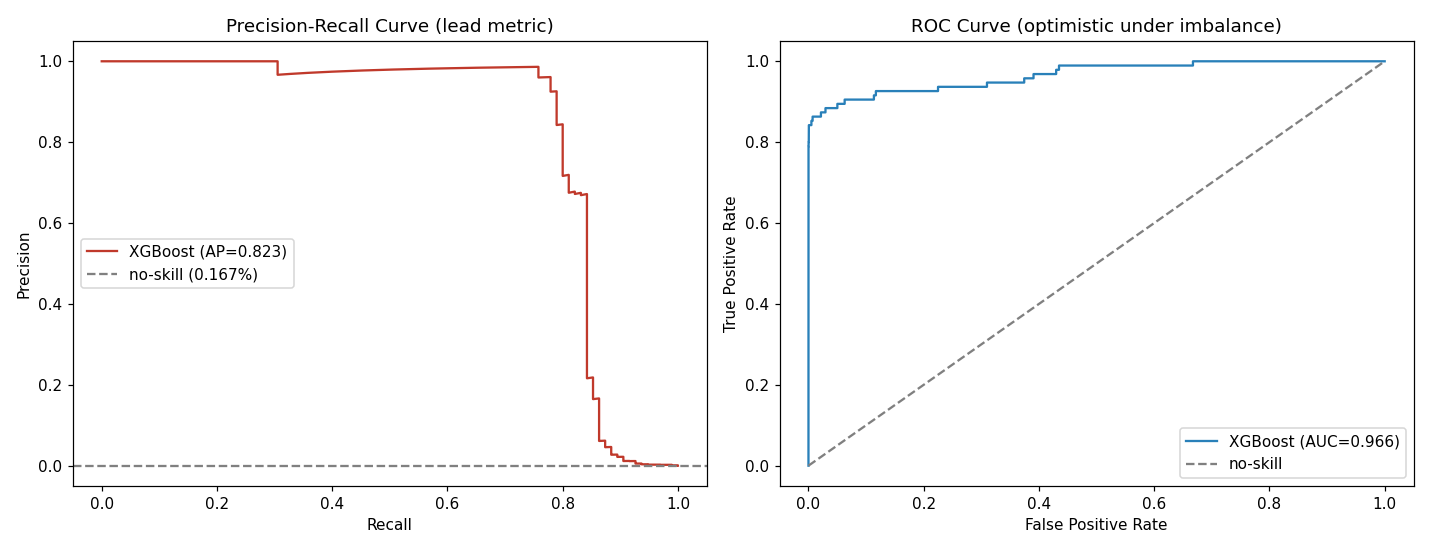
\includegraphics[width=0.95\textwidth]{06_pr_roc_curves.png}
\caption{Precision--Recall curve (lead) and ROC curve (context) for XGBoost.}
\end{figure}

We swept thresholds against an explicit cost model --- a missed fraud (FN) costs
\$150, a false alarm (FP) costs \$5 (illustrative; real figures would come from
finance) --- and minimised total cost.

\begin{figure}[H]
\centering
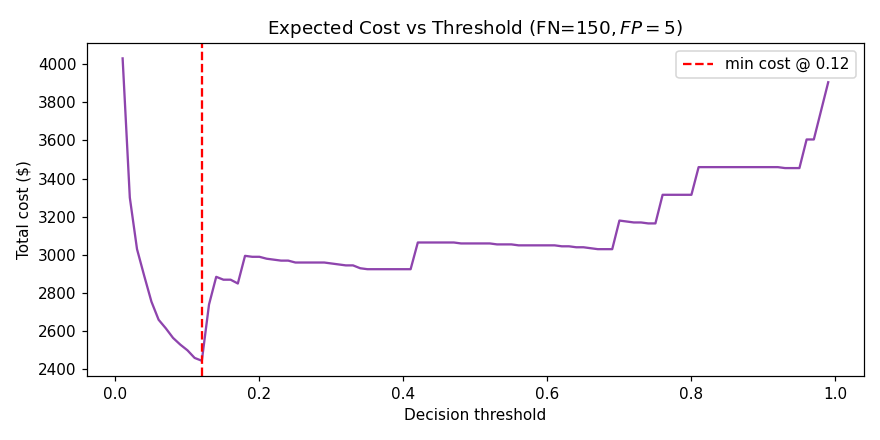
\includegraphics[width=0.75\textwidth]{07_cost_vs_threshold.png}
\caption{Total expected cost as a function of the decision threshold.}
\end{figure}

\begin{table}[H]
\centering
\caption{Threshold strategies and their business outcomes.}
\begin{tabular}{@{}lrrrrrrr@{}}
\toprule
\textbf{Strategy} & \textbf{Thr.} & \textbf{TP} & \textbf{FN} & \textbf{FP} &
\textbf{Recall} & \textbf{Prec.} & \textbf{Cost} \\
\midrule
Default & 0.50 & 75 & 20 & 12 & 79\% & 86\% & \$3{,}060 \\
Max recall & 0.0006 & 86 & 9 & 3{,}558 & 91\% & 2.4\% & \$19{,}140 \\
\textbf{Cost-optimal} & \textbf{0.12} & 80 & 15 & 39 & 84\% & 67\% & \textbf{\$2{,}445} \\
\bottomrule
\end{tabular}
\end{table}

\begin{figure}[H]
\centering
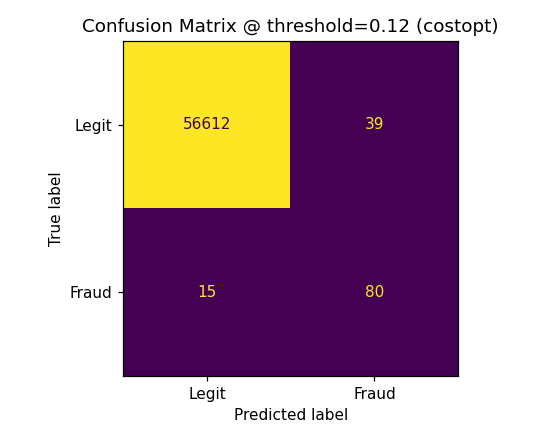
\includegraphics[width=0.55\textwidth]{08_confusion_costopt.png}
\caption{Confusion matrix at the cost-optimal threshold (0.12).}
\end{figure}

\paragraph{Interpretation.} Lowering the threshold to 0.12 catches 5 more frauds
than the default for 27 more reviews --- worthwhile because a missed fraud costs
$\sim$30$\times$ a false alarm, cutting estimated cost $\sim$20\%. Chasing maximum
recall is counter-productive: it triggers 3{,}558 false alarms and sextuples cost.

%------------------------------------------------------------------------------
\section{Business Recommendation}
\begin{enumerate}[leftmargin=1.5em]
  \item \textbf{Deploy XGBoost at the 0.12 threshold} --- best balance of fraud
        caught vs.\ review workload under the stated cost assumptions.
  \item \textbf{Replace placeholder costs} with finance's real FN/FP figures and
        re-tune; the optimal threshold is a direct function of them.
  \item \textbf{Pilot in shadow mode} (score live traffic without acting) before
        any automated decline.
  \item \textbf{Layer with simple rules} (e.g.\ extra scrutiny on 2--4\,AM
        transactions) for defence in depth.
  \item \textbf{Monitor for drift and retrain} on a schedule --- fraud tactics
        evolve.
\end{enumerate}

%------------------------------------------------------------------------------
\section{Limitations}
\begin{itemize}[leftmargin=1.4em]
  \item \textbf{Offline analysis}, not a production system --- no real-time scoring
        or monitoring.
  \item \textbf{Concept drift:} performance decays as fraud patterns change.
  \item \textbf{Anonymised features} preclude business-level explanation and
        regulatory reason-codes.
  \item \textbf{Small fraud sample} ($\sim$378 train cases) caps learnable signal;
        SMOTE cannot invent genuinely new fraud types.
  \item \textbf{Cost assumptions are placeholders} that drive the threshold
        recommendation.
  \item \textbf{One region, two days} --- not representative of all fraud or
        seasonality.
\end{itemize}

%------------------------------------------------------------------------------
\section{Reproducibility}
\begin{verbatim}
pip install -r requirements.txt     # macOS XGBoost: also `brew install libomp`
# place creditcard.csv in data/raw/
python src/preprocessing.py         # clean + leak-safe splits
python src/models.py                # train & compare, saves best model
python src/evaluate.py              # curves + threshold tuning
# or run notebooks/01_eda, 02_eda_deep, 03_modeling end to end
\end{verbatim}

%------------------------------------------------------------------------------
\section{Conclusion and Next Steps}
The project delivers a complete, honest fraud-analytics workflow: from a 0.17\%
needle-in-a-haystack problem to a cost-aware deployment recommendation. The
standout analytical results are the \textbf{2--4\,AM fraud spike}
($\sim$8$\times$), the \textbf{PR-AUC-vs-ROC-AUC lesson} (ROC 0.97 hiding 5.6\%
precision), and the \textbf{cost-based threshold} that converts a probability into
a $\sim$20\% cost reduction. Next we will apply the same pipeline to the
\textbf{PaySim} dataset, whose readable columns allow genuinely interpretable
feature engineering, and build a Streamlit dashboard exposing the threshold slider
interactively.

\end{document}
